% !TEX root = main.tex
% Main text: abstract through conclusion. Formal assumptions, full statements and proofs are in the appendix.
\begin{abstract}
A Transformer can represent a counting algorithm and still struggle to learn it from final answers. On counting modulo a small number,
showing the running counts makes the task much easier to learn. We explain this gap through the information each training signal carries.
Every letter hidden from a feature contracts its correlation with the final count, while near initialization the Transformer's output is
dominated by features that read only a few letters. A displayed count exposes the next update directly. In a two-block Transformer that
holds exact solutions for both formats, outcome gradient flow from a zero readout stays near chance for a time exponential in the number
of letters. With a gate that reads the displayed count and the current letter, joint gradient flow from zero readouts and small nonzero
gate scalars along fixed structured directions reaches positive margins on every transition in polynomial time. This holds for every modulus when match and
non-match probabilities differ; the proof supplies the routing and gate-readout direction. A clean binary extension also learns
soft suppression of designated zero-key, zero-value distractors from diffuse attention in polynomial time.
A full-prefix extension learns the current-letter relative offset within a tied feature family and reaches a prescribed step loss with fixed group mobilities.
Experiments test what happens beyond these restrictions: step supervision helps on counting,
other state-tracking tasks, and LoRA-tuned Qwen2.5-0.5B on BIG-Bench Hard object tracking. It does not help at every size, and one reversal
remains unexplained.

\end{abstract}

% ===================================================================
\section{Introduction}
\label{sec:intro}

A model that can count need not learn to count from final answers. In our experiments, the same Transformer succeeds when shown
running counts and stays near chance when trained on the final count alone. Yet we can write down exact parameters for either
computation. If both solutions are available, what does showing the steps give the learner?

Intermediate supervision often makes reasoning tasks easier to learn \citep{nye2021scratchpads,wei2022cot,lightman2023verify}.
The usual intuition is that steps break a long computation into smaller ones. We ask what this means for the gradient of a fixed
network. Counting a query letter modulo $K$ lets us examine that question closely: the answer-only and step-by-step tasks share the
same counting process, architecture, initialization and training budget (\cref{fig:chain}b, \cref{fig:overview}a).

The key is what a feature learns from the letters it reads. Averaging over every other letter contracts its correlation with the
final count by a factor $\mixrate<1$ per unseen letter. Near initialization, the output is dominated by terms that each read one letter;
combining more letters costs powers of the initialization scale (\cref{fig:overview}b). Final answers thus supply very little credit
to the features the network can readily change. A displayed count and the current letter, however, expose the next update. The two paths are
{\small
\[
\begin{aligned}
 &\text{outcome:}&&\text{hidden letters}\to\text{few-letter features decorrelate}\to\text{tiny credit}\to\text{plateau},\\
 &\text{step:}&&\text{displayed count}\to\text{local innovation}\to\text{accessible credit}\to\text{learned transition}\to\text{solution}.
\end{aligned}
\]
}

\begin{figure}[t]
\centering
%% Figure 1 (pgfplots). Data: results/paper/zero_readout_n16_8k (seeds 42-51, median and 25th-75th percentile band),
%% results/paper/fig2/n8_s42.json (target A_r) and results/paper/exact_spectra/sigma_sweep/s42_sg0.02.txt (Jacobian J_r).
\definecolor{stepc}{HTML}{0072B2}\definecolor{outc}{HTML}{D55E00}\definecolor{theoc}{HTML}{009E73}
\definecolor{modelc}{HTML}{7B4F9E}\definecolor{mutedc}{HTML}{6E6E6E}
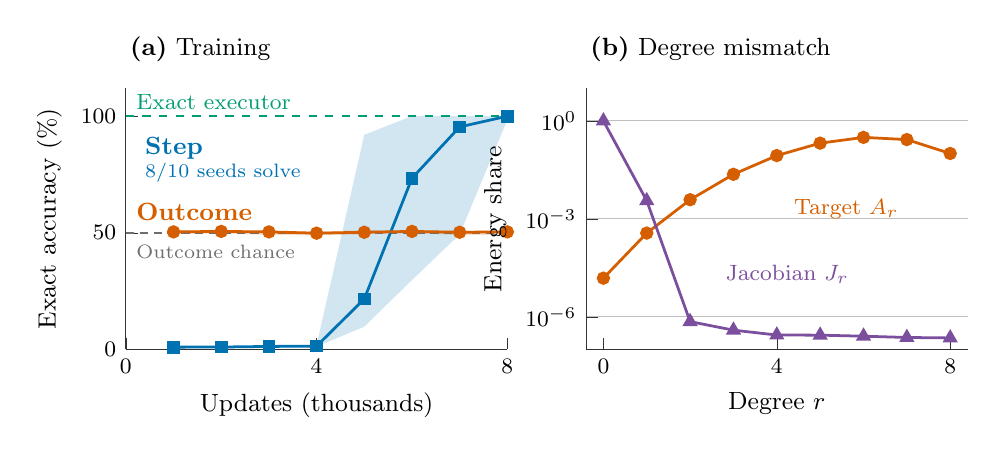
\begin{tikzpicture}
\pgfplotsset{every axis/.style={width=0.53\linewidth, height=4.9cm, axis line style={black!80}, tick style={black!80},
  tick label style={font=\footnotesize}, label style={font=\small}, title style={font=\small, at={(0,1)}, anchor=south west, xshift=-2pt}},
  every axis plot/.append style={line width=1pt}}
\begin{axis}[name=train, title={\textbf{(a)} Training}, xlabel={Updates (thousands)}, ylabel={Exact accuracy (\%)},
  xmin=0, xmax=8, ymin=0, ymax=112, xtick={0,4,8}, ytick={0,50,100}, axis x line*=bottom, axis y line*=left, clip=false]
  \addplot[draw=none, fill=stepc, fill opacity=0.18, forget plot] coordinates {(1,0.55) (2,0.73) (3,0.82) (4,1.25) (5,9.77) (6,29.75) (7,49.33) (8,98.40) (8,100.00) (7,100.00) (6,100.00) (5,92.03) (4,1.90) (3,1.40) (2,1.35) (1,1.35)};
  \addplot[draw=none, fill=outc, fill opacity=0.18, forget plot] coordinates {(1,49.52) (2,49.73) (3,49.05) (4,48.92) (5,49.35) (6,49.92) (7,48.97) (8,49.15) (8,50.70) (7,50.70) (6,51.20) (5,51.08) (4,50.60) (3,50.70) (2,51.08) (1,51.08)};
  \addplot[theoc, dashed, line width=0.9pt, domain=0:8, samples=2] {100};
  \addplot[mutedc, densely dashed, line width=0.8pt, domain=0:8, samples=2] {50};
  \addplot[stepc, mark=square*, mark size=1.8pt] coordinates {(1,1.00) (2,1.05) (3,1.30) (4,1.45) (5,21.65) (6,73.40) (7,95.40) (8,100.00)};
  \addplot[outc, mark=*, mark size=1.9pt] coordinates {(1,50.40) (2,50.60) (3,50.40) (4,49.85) (5,50.25) (6,50.60) (7,50.25) (8,50.40)};
  \node[anchor=south west, font=\footnotesize, text=theoc, inner sep=1pt] at (axis cs:0.15,101.5) {Exact executor};
  \node[anchor=west, font=\small\bfseries, text=stepc] at (axis cs:0.2,86) {Step};
  \node[anchor=west, font=\scriptsize, text=stepc] at (axis cs:0.2,76) {8/10 seeds solve};
  \node[anchor=south west, font=\small\bfseries, text=outc, inner sep=1pt] at (axis cs:0.15,54) {Outcome};
  \node[anchor=north west, font=\scriptsize, text=mutedc, inner sep=1pt] at (axis cs:0.15,46) {Outcome chance};
\end{axis}
\begin{semilogyaxis}[at={(train.east)}, anchor=west, xshift=1.0cm, title={\textbf{(b)} Degree mismatch}, xlabel={Degree $r$},
  ylabel={Energy share}, xmin=-0.4, xmax=8.4, ymin=1e-7, ymax=10, xtick={0,4,8}, ytick={1e-6,1e-3,1},
  ymajorgrids, major grid style={black!25}, axis x line*=bottom, axis y line*=left]
  \addplot[outc, mark=*, mark size=1.9pt] coordinates {(0,1.5259e-05) (1,3.6621e-04) (2,3.8452e-03) (3,2.3071e-02) (4,8.6517e-02) (5,2.0764e-01) (6,3.1146e-01) (7,2.6697e-01) (8,1.0011e-01)};
  \addplot[modelc, mark=triangle*, mark size=2.2pt] coordinates {(0,9.9641e-01) (1,3.5840e-03) (2,7.1281e-07) (3,3.9081e-07) (4,2.7680e-07) (5,2.7450e-07) (6,2.5510e-07) (7,2.3310e-07) (8,2.2560e-07)};
  \node[anchor=north, font=\footnotesize, text=outc] at (axis cs:5.6,8e-3) {Target $A_r$};
  \node[anchor=west, font=\footnotesize, text=modelc] at (axis cs:2.6,2e-5) {Jacobian $J_r$};
\end{semilogyaxis}
\end{tikzpicture}

\caption{\textbf{Same architecture and task, different training behavior.}
(a)~Counting with $n=16$, $K=2$ and zero readout: median exact continuation accuracy and interquartile band over ten paired seeds, $8$k
updates; the dashed line marks the exact executor that both formats admit (\cref{prop:represent}).
(b)~A separate $n=8$, $K=2$, $\initscale=0.02$ measurement with nonzero readout: target and Jacobian energy occupy different ANOVA degrees, the number of letters a component depends on jointly (\cref{app:spectrum}).}
\label{fig:overview}
\end{figure}

\needspace{3\baselineskip}
\paragraph{Contributions.}
\begin{itemize}[leftmargin=*,itemsep=2pt,topsep=3pt]
\item \textbf{Unseen letters erase outcome credit} (\cref{sec:credit}). A feature that reads a set $S$ of letters has correlation at most
$\mixrate^{n-|S|}$ with the final count, so near initialization outcome credit decays like $\mixrate^n$; the upper bound and leading coefficient of
step credit for the counting rule carry no such factor (\cref{thm:main,thm:separation}).
\item \textbf{Outcome training plateaus} (\cref{thm:outcome-end}). From a zero readout, gradient flow stays near chance under any block schedule, the relative bias included,
for time $\Omega(\mixrate^{-n})$, in a Transformer wide enough to hold the outcome executor.
\item \textbf{Step training converges} (\cref{thm:joint}). For a gate head that reads the displayed count and the current
letter, joint gradient flow on its query and key scalars and both readouts, from zero readouts and small nonzero scalars along fixed structured directions,
reaches positive margins on every count in a time polynomial in the inverse initialization scale and the head dimension, with no other dependence on $n$.
A clean binary extension jointly learns distractor penalties, shared or independent, and enters a useful routing region before completing the transitions.
\item \textbf{Experiments} (\cref{sec:experiments}) test each prediction: the exponential plateau, outcome accuracy at the
low-degree prior, learnable routing, and step supervision beyond counting, including a pretrained model.
\end{itemize}

\Cref{sec:related} places this fixed-target comparison alongside work on parity and intermediate supervision.

% ===================================================================
\section{Setup}
\label{sec:setup}
\label{sec:setting}

Modular counting keeps the state space fixed as the prompt grows. What increases is the number of updates hidden behind the
answer. We can therefore lengthen the computation without changing the prediction problem at its end.

\begin{definition}[Counting modulo $K$]
\label{def:task}
A prompt has a start count $s_0$, uniform on $\mathbb Z_K$, and letters $w_1,\ldots,w_n$ drawn i.i.d.\ from an alphabet
in which a fixed query letter $w^\star$ has probability $p\in(0,1)$. With $b_t=\mathbf 1[w_t=w^\star]$,
\begin{equation}
 s_t=s_{t-1}+b_t\pmod K,\qquad t=1,\ldots,n,
 \label{eq:tracking}
\end{equation}
and the answer is $y=s_n$.
\end{definition}

\begin{definition}[Contraction coefficient]
\label{def:lambda}
For counting modulo $K$,
\begin{equation}
 \mixrate=\max_{1\le j<K}\bigl|1-p+p\,e^{2\pi\mathrm ij/K}\bigr|=\bigl|1-p+p\,e^{2\pi\mathrm i/K}\bigr|.
 \label{eq:lambda}
\end{equation}
\end{definition}

\begin{figure}[t]
\centering
\resizebox{\linewidth}{!}{% Conceptual figure: counting modulo K as a cyclic chain, and what each supervision format sees.
\begin{tikzpicture}[>=Stealth, font=\small,
  state/.style={circle, draw=royalazure!80!black, fill=royalazure!12, minimum size=7mm, inner sep=0pt},
  tok/.style={rectangle, rounded corners=2pt, draw=black!45, fill=black!4, minimum width=7mm, minimum height=5.5mm, inner sep=1pt},
  sup/.style={rectangle, rounded corners=2pt, draw=royalazure!80!black, fill=royalazure!12, minimum width=7mm, minimum height=5.5mm, inner sep=1pt},
  hid/.style={rectangle, rounded corners=2pt, draw=black!30, dashed, fill=white, text=black!45, minimum width=7mm, minimum height=5.5mm, inner sep=1pt}]

% ---------------- (a) cyclic chain ----------------
\begin{scope}[shift={(0,0)}]
  \foreach \i/\lab in {0/0, 1/1, 2/2, 3/{K{-}1}} {
    \node[state] (c\i) at ({90-\i*90}:1.25) {$\lab$};
  }
  \foreach \i/\dir in {0/90, 1/0, 2/-90, 3/180} {
    \draw[->, black!55] (c\i) to[out=\dir+28, in=\dir-28, looseness=6] node[pos=0.5, font=\scriptsize, fill=white, inner sep=0.5pt] {$1{-}p$} (c\i);
  }
  \draw[->, thick, royalazure] (c0) to[bend left=22] node[font=\scriptsize, above right=-1pt] {$p$} (c1);
  \draw[->, thick, royalazure] (c1) to[bend left=22] node[font=\scriptsize, below right=-1pt] {$p$} (c2);
  \draw[->, thick, royalazure, dashed] (c2) to[bend left=22] node[font=\scriptsize, below left=-1pt] {$p$} (c3);
  \draw[->, thick, royalazure] (c3) to[bend left=22] node[font=\scriptsize, above left=-1pt] {$p$} (c0);
  \node[align=center, font=\footnotesize] at (0,-2.6)
    {$s_t=s_{t-1}+b_t\ (\mathrm{mod}\ K)$\\[2pt] $\mathbf T=(1-p)\,\mathbf I+p\,\mathbf R$};
  \node[font=\small\bfseries] at (-2.3,1.75) {(a)};
\end{scope}

% ---------------- (b) what each format supervises ----------------
\begin{scope}[shift={(3.4,0.95)}]
  \node[font=\small\bfseries] at (-0.35,0.8) {(b)};
  % outcome row
  \node[anchor=west, font=\footnotesize] at (0,0.8) {Outcome: supervise $s_n$ only};
  \node[tok] (o0) at (0.45,0) {$s_0$};
  \node[tok] (ow1) at (1.35,0) {$w_1$};
  \node[hid] (os1) at (2.25,0) {$s_1$};
  \node[tok] (ow2) at (3.15,0) {$w_2$};
  \node[hid] (os2) at (4.05,0) {$s_2$};
  \node at (4.85,0) {$\cdots$};
  \node[tok] (own) at (5.65,0) {$w_n$};
  \node[sup] (osn) at (6.55,0) {$s_n$};
  \draw[decorate, decoration={brace, amplitude=4pt, mirror}, black!60] (1.0,-0.42) -- (6.0,-0.42)
    node[midway, below=4pt, font=\footnotesize, align=center] {$n$ hidden letters: each Fourier mode contracts by $\le\mixrate$ per letter};
  % step row
  \node[anchor=west, font=\footnotesize] at (0,-1.75) {Step: supervise every $s_t$ from the displayed $s_{t-1}$};
  \node[tok] (p0) at (0.45,-2.55) {$s_0$};
  \node[tok] (pw1) at (1.35,-2.55) {$w_1$};
  \node[sup] (ps1) at (2.25,-2.55) {$s_1$};
  \node[tok] (pw2) at (3.15,-2.55) {$w_2$};
  \node[sup] (ps2) at (4.05,-2.55) {$s_2$};
  \node at (4.85,-2.55) {$\cdots$};
  \node[tok] (pwn) at (5.65,-2.55) {$w_n$};
  \node[sup] (psn) at (6.55,-2.55) {$s_n$};
  \draw[rounded corners=3pt, thick, lightmauve!80!black] (1.83,-2.95) rectangle (3.55,-2.15);
  \draw[->, thick, lightmauve!80!black] (3.55,-2.55) -- (ps2.west);
  \node[font=\footnotesize, align=center] at (3.5,-3.45) {one local transition $(s_{t-1},w_t)\mapsto s_t$: innovation $\ge1-\mixrate^2$};
\end{scope}
\end{tikzpicture}
}
\caption{\textbf{One counting process, two views of it.}
(a)~Counting modulo $K$ is a cyclic Markov chain: each letter keeps the count with probability $1-p$ and advances it with probability
$p$, so the transition matrix is $\mathbf T=(1-p)\mathbf I+p\mathbf R$ with $\mathbf R$ the cyclic shift. Its nonconstant Fourier modes
contract by at most $\mixrate$ per step (\cref{app:contraction}).
(b)~Outcome supervision labels only $s_n$, so the label depends on the letters through $n$ unseen steps of the chain and its
correlation with any feature of $k$ letters shrinks like $\mixrate^{n-k}$ (\cref{thm:main}). Step supervision displays $s_{t-1}$ and labels $s_t$, so each label is one
step of the chain and keeps an innovation of at least $1-\mixrate^2$ (\cref{thm:separation}).}
\label{fig:chain}
\end{figure}

Averaging over one unseen letter contracts every nonconstant Fourier mode of the count by at most $\mixrate$ (\cref{fig:chain}); in information-theoretic terms,
$\mixrate$ is the maximal correlation of consecutive counts and $\mixrate^2$ the $\chi^2$ contraction coefficient of one
unseen letter \citep{witsenhausen1975sequences,raginsky2016strong}. The complementary quantity $1-\mixrate^2$ is the
variance a displayed count leaves to the next letter (\cref{eq:local-variation}). For four uniform letters,
$\mixrate=0.5$ at $K=2$ and $0.66$ at $K=3$.

\paragraph{Formats.} Both formats see the same prompt. The \emph{outcome loss} $\Lout$ is the cross-entropy of the final
count; the \emph{step loss} $\Lstep$ is the teacher-forced cross-entropy of the transitions $s_{t-1},w_t\mapsto s_t$ for
$t\ge2$; the first prediction is a boundary case whose previous count sits in the prompt (\cref{def:losses}). Experiments
supervise every running count unless stated otherwise.

\paragraph{Model.} A causal Transformer with two blocks of softmax heads and ReLU MLPs, a relative position bias
initialized at zero, no LayerNorm, arbitrary widths and a linear readout (\cref{ass:arch}), initialized at
$\bm\theta_0=\initscale\tilde{\bm\theta}$ with fan-in operator-norm bounds and MLP biases of order one (\cref{ass:init}). The biases fix
every ReLU's sign on a ball $\initball$ of radius proportional to $\initscale$, provided
$\initscale\le\initscale_0=c\min(1,\frac{1}{N_b})$ with $N_b$ the MLP bias norm (of order $\sqrt n$ at executor width, \cref{rem:end-width}), so near initialization the MLPs act linearly;
the AdamW experiments drop this condition (\cref{rem:two-block-bias}). Constants $c,C$ depend on neither the widths, $n$ nor
$\initscale$.

\begin{proposition}[Both solutions exist]
\label{prop:represent}
For every $K$, alphabet size and $n$, one architecture as in \cref{ass:arch}, with widths linear in $n$, has parameters
$\thstep$ and $\thout$ at which greedy decoding produces the correct step and outcome continuations on every prompt, with
a positive logit margin.
\end{proposition}

\subsection{Two exact programs in one Transformer}
\label{sec:exact-programs}
The exact executors make the training failure more puzzling. One program updates the state locally; the other aggregates the match
bits before applying modular arithmetic. Both fit in this Transformer. We still have to explain why training reaches one so much
more readily than the other.

\begin{center}
\small
\begin{tabular}{@{}llll@{}}
\toprule
Executor & Block 1 & Block 2 & Output (lookup, modulo $K$)\\
\midrule
Step & $b_t=\mathbf 1[w_t=w^\star]$ & route $s_{t-1}$ and $b_t$ & $s_t=s_{t-1}+b_t$\\
Outcome & every $b_t$ & average $b_1,\ldots,b_n$; route $s_0$ & $s_n=s_0+\sum_tb_t$\\
\bottomrule
\end{tabular}
\end{center}
Two primitives implement them: positional attention with scores of order $\log n$ on a chosen source set copies one register or
averages several, and one ReLU unit per count--bit pair performs the modular lookup. Routing leakage is $O(n^{-2})$;
\cref{app:architectures} gives the literal tensor entries and the error calculation, certifying a logit margin greater than $19$ on every
prompt.

% ===================================================================
\section{Credit through unseen letters}
\label{sec:credit}

To understand the training gap, we first ask how much information about the target reaches a parameter update.
Fix the start count, so the letters are independent.

\begin{definition}[Credit]
\label{def:credit}
For a target signal $\bm\xi$, a random vector in $\R^K$, let $\cred_{\bm\xi}(\bm\theta)=\E[\langle\bm z_{\bm\theta},\bm\xi\rangle]$. The
\emph{credit} for $\bm\xi$ is $\|\nabla_{\bm\theta}\cred_{\bm\xi}\|=\bigl\|\E\bigl[(\Jz)^\top\bm\xi\bigr]\bigr\|$.
\end{definition}

For the outcome signal $\bm\xi=\bm y-\bm u$ (one-hot answer minus uniform), credit is the answer-dependent part of the gradient of
$\Lout$ (\cref{lem:gradient-split}; \citealp{shalevshwartz2017failures,abbe2025parities}).

\subsection{Outcome: few-letter features cannot see the final count}
\paragraph{What a feature misses.} Suppose a feature $\mathbf H$ reads only the letters in a set $S$. Even if it uses those letters perfectly,
it must average over every letter outside the set. By the tower property,
$\E[\mathbf H^\top(\bm y-\bm u)]=\E[\mathbf H^\top\E[\bm y-\bm u\mid w_S]]$, and given $w_S$ the $n-|S|$ unseen letters still move the count: each
multiplies every nonconstant Fourier mode of its distribution by at most $\mixrate$ (\cref{fig:chain}a). Hence
\begin{equation}
 \bigl\|\E\bigl[\mathbf H^\top(\bm y-\bm u)\bigr]\bigr\|\le\mixrate^{n-|S|}\,\|\mathbf H\|_{L^2}
 \label{eq:credit-degree}
\end{equation}
(\cref{lem:target-contraction}). Each omitted letter has the same multiplicative cost; seeing a few letters cannot bypass the rest of
the computation. The exponent is sharp.

\paragraph{The network reads few letters at a time.} Scale every attention score by $\zeta\in[0,1]$ and expand in $\zeta$. At $\zeta=0$ attention is uniform
and the MLPs are affine, so the network is additive over positions: each term reads at most one letter. Every interaction among letters
passes through the scores, and a term with $k\ge1$ scores reads at most $2k+1$ letters and costs $\initscale^{2+4k}$ in the Jacobian
(\cref{prop:score-degree}). Applying \cref{eq:credit-degree} term by term bounds the outcome credit. Call the credit of the score-dependent part
$\mathbf J_{\mathrm{score}}$ of the Jacobian the \emph{score-mediated credit}: it contains every term that reads two or more letters, and
also score-dependent terms that read one.

\begin{theorem}[Unseen letters erase outcome credit]
\label{thm:main}
Under \cref{ass:arch,ass:init,ass:task}, with the start count fixed:
\begin{enumerate}[label=(\roman*),leftmargin=*,itemsep=0pt,topsep=2pt]
\item for every set $S$ of letters and every square-integrable $\mathbf H$ that depends only on the letters in $S$, \cref{eq:credit-degree} holds;
\item for all $n\ge2$, $\initscale^2\le c\mixrate$ and $\bm\theta\in\initball$, the score-mediated credit is at most $C\initscale^6\mixrate^{n-3}$, and if
$\initscale\le c\mixrate$ the whole outcome credit is at most $C\initscale\mixrate^n$.
\end{enumerate}
\end{theorem}

\subsection{Step: a local innovation survives}
A large step gradient could be misleading. The displayed count alone predicts the two possible next states and their probabilities.
Fitting that prior lowers the loss without learning how to use the current letter. We separate that easy signal from the rule itself. With the
state-only predictor $\bm q_s=(1-p)\bm e_s+p\,\bm e_{s+1}$, write $\bm e_{s_t}-\bm u=(\bm q_{s_{t-1}}-\bm u)+\bm g_t$, where the
\emph{rule signal}
\[
 \bm g_t=\bm e_{s_t}-\bm q_{s_{t-1}}=(b_t-p)\bigl(\bm e_{s_{t-1}+1}-\bm e_{s_{t-1}}\bigr)
\]
has covariance, on the centred state subspace $\one^\perp:=\{v\in\R^K:\one^\top v=0\}$,
\begin{equation}
 \operatorname{Cov}(\bm g_t)\succeq\frac{1-\mixrate^2}{K}\,I
 \quad\text{on }\one^\perp.
 \label{eq:local-variation}
\end{equation}
Thus an outcome target pays $\mixrate^{n-|S|}$ for the letters a feature does not read, whereas a displayed transition pays the
local innovation $1-\mixrate^2$ only once. Let $\rulecredit$ be the credit
functional with the rule signal as target.

\begin{theorem}[Step credit]
\label{thm:separation}
Under \cref{ass:arch,ass:init,ass:task} with a uniform start, for all $n\ge2$ and $\bm\theta\in\initball$:
\begin{enumerate}[label=(\roman*),leftmargin=*,itemsep=0pt,topsep=2pt]
\item \emph{(prior-fitting gradient)} if $\initscale\le c\mixrate$, then $\|\nabla_{\bm\theta}\Lstep(\bm\theta)\|\ge c\,\initscale\mixrate$ while
$\|\nabla_{\bm\theta}\Lout(\bm\theta)\|\le C\initscale(\initscale^2+\mixrate^n)$;
\item \emph{(rule credit)} if $\initscale\le c$ and attention uses the full causal prefix, then $\|\nabla_{\bm\theta}\rulecredit(\bm\theta)\|\le \frac{C\initscale^6}{n}$; if
moreover $p<\tfrac{1}{2}$, the degree-$6$ polynomial $P_n$ is not identically zero, with an explicit count$\times$letter monomial of
coefficient of order $\frac{1}{n\sqrt{d_{\mathrm h}}}$
(\cref{lem:leading}).
\end{enumerate}
\end{theorem}

Part~(i) fits the count-only prior. Part~(ii) isolates the rule signal: its upper bound is of order $\frac{\initscale^6}{n}$, without
the factor $\mixrate^n$, and its nonzero leading coefficient shows that the signal can survive. Its size at random initialization
remains a separate question. The bound becomes two-sided at any direction with
$|P_n(\tilde{\bm\theta})|\ge\frac{\rulemargin}{n}$, where $\|\nabla_{\bm\theta}\rulecredit(\initscale\tilde{\bm\theta})\|\ge\frac{\initscale^6\rulemargin}{2n}$ for
$\initscale\le c\min(\rulemargin\initscale_0,\rulemargin^{1/4})$ (\cref{rem:generic-rule}); we do not prove such a margin at random
initialization. Measurements are in \cref{app:regime}.

% ===================================================================
\section{Which solution training reaches}
\label{sec:reach}

Small initial credit alone does not imply slow learning: the parameters might reach a region with a stronger signal. We ask
whether outcome flow can get there quickly, and whether step flow can turn its local signal into a learned transition.

\subsection{Outcome: an exponential plateau}

The next theorem controls the trajectory as it tries to leave initialization. A local loss floor limits how far gradient flow can travel.

\begin{theorem}[Exponential-time outcome plateau near small initialization]
\label{thm:outcome-end}
Under \cref{ass:arch,ass:init,ass:task} with a zero initial readout, let $P(t)$ be, at each time, the orthogonal projection onto a set
of trainable parameter blocks, piecewise constant in $t$; the blocks may include the relative bias. Consider gradient flow
$\tfrac{d\bm\theta}{dt}=-\mathbf P(t)\nabla_{\bm\theta}\Lout(\bm\theta)$; full joint flow ($\mathbf P\equiv\mathbf I$) and training only the blocks of \cref{thm:joint} are special cases.
For all $n\ge2$, $\initscale\le c\mixrate$ and $0\le t\le c\mixrate^{-n}$, with constants that do not depend on the schedule:
\begin{enumerate}[label=(\roman*),leftmargin=*,itemsep=0pt,topsep=2pt]
\item \emph{(locality)} $\|\bm\theta(t)-\bm\theta_0\|\le\ballradius\initscale$, the relative bias included in the norm;
\item \emph{(loss)} $\Lout(\bm\theta(t))\ge\log K-C\initscale^2\mixrate^n$;
\item \emph{(correct-answer probability)} $\E\bigl[\softmax(\bm z_{\bm\theta(t)})_y\bigr]\le\frac{1}{K}+C\initscale\mixrate^{n/2}$.
\end{enumerate}
\end{theorem}
The theorem bounds the length of the plateau; it does not assert that outcome training never converges.

\emph{Proof idea.} Along the flow, for any schedule,
\[
 \frac{d\Lout}{dt}=-\|\mathbf P(t)\nabla_{\bm\theta}\Lout\|^2,
 \qquad\text{so}\qquad
 \|\bm\theta(t)-\bm\theta_0\|^2\le t\,\bigl(\Lout(\bm\theta_0)-\Lout(\bm\theta(t))\bigr).
\]
This gives the weak signal a consequence beyond the first update. Near $\bm\theta_0$, the outcome loss can fall by at most
$C\initscale^2\mixrate^n$ (\cref{lem:score-sum}), even with a trained relative bias (\cref{lem:bias-uniform}). That small decrease limits
the distance the flow can travel: leaving the ball takes time of order $\mixrate^{-n}$ (\cref{app:end}).

\subsection{Step: joint gradient flow learns the transition}
\label{sec:step}
For step training, we first isolate learning the transition with supplied routing, and then allow the gate to learn
soft suppression of distractors in a clean binary model. Both results use a small structured interaction and zero readouts;
the second starts with diffuse attention and proves entry into a useful routing region.

\paragraph{Scores and features.} The gate reads the displayed count at $i_t$ and the current letter at $j_t$.
The supplied-routing model admits only these two sites. The clean model additionally admits $m\ge1$ designated distractors,
each with zero key and value, and assigns them one shared trainable penalty $B$:
\begin{equation}
 \begin{gathered}
 \mathrm{score}(i_t)=0,\qquad \mathrm{score}(j_t)=(-1)^{b_t}a,\qquad
 \mathrm{score}(\text{distractor})=-B,\\
 r_b=\frac{1}{1+e^{(-1)^ba}+me^{-B}}.
 \end{gathered}
 \label{eq:J-clean-scores}
\end{equation}
For supplied routing, set $m=0$, giving $r_b=\sigma(-(-1)^ba)$. In either model the logits are
\[
 \bm z_t=\initscale\mathbf U\bm x_t+\initscale v r_{b_t}\mathbf W\bm x_t,
 \qquad \bm x_t=\bm e_{s_{t-1}},\qquad a=\frac{\initscale^2qk}{\sqrt{d_{\mathrm h}}},
\]
with count readout $\mathbf U$ and gate readout $\mathbf W=w(\mathbf I-\mathbf R)$.
The query, key and value directions read the count, read the letter and carry the count, respectively
(\cref{app:joint}).

\paragraph{Initialization and training.} Both readouts start at zero and
$\initscale/2\le |q(0)|,|k(0)|,|v|\le2\initscale$, so the initial prediction is uniform and
$|a(0)|$ is of order $\initscale^4$. One simultaneous Euclidean gradient flow trains $\mathbf U,\mathbf W,q,k$,
with $v$ and all other maps fixed. The gate readout stays on its transition line (no restriction for $K=2$).
For supplied routing, the scalar signs may be arbitrary. For the clean model, $K=2$, $0<p<1/2$,
$q(0)k(0)<0$, and $B(0)=\delta\in[0,1]$. The flow also trains $B$ with mobility $\nu\in(0,1]$:
$\dot B=-\nu\,\partial_B\Lstep$. A Euclidean scalar penalty has $\nu=1$;
tying $m$ bias entries to $-B$ under their Frobenius metric has $\nu=1/m$.
The useful-site biases stay zero. At $\delta=0$ there is no initial bias advantage over the distractors.

\begin{theorem}[Joint transition learning and clean routing]
\label{thm:joint}
\textnormal{(i) Supplied routing.} Count modulo $K\ge2$ with $n\ge2$ letters and a query of probability $p\in(0,1)$, $p\neq\tfrac{1}{2}$, and let $h^\star=|\log\tfrac{1-p}{p}|$,
$p_{\min}=\min(p,1-p)$ and $\mathrm{gap}\in(0,1]$. Call the initialization \emph{aligned} if $q(0)k(0)(1-2p)<0$ and \emph{misaligned} otherwise.
For $\initscale$ below the explicit threshold in \cref{app:J-constants}, and in the misaligned case
$|\qkbalance|\ge\mathrm{gap}\,\initscale^2$ with $\qkbalance=q(0)^2-k(0)^2$, joint gradient flow on $\Lstep$ gives
every prediction positive margin against all $K-1$ other counts at every time $t\ge T$, and $\Lstep\to0$, where, with an absolute constant $C$,
$\gamma=\mathrm{gap}$ (misaligned) or $\gamma=1$ (aligned),
\[
 T\le\frac{C}{\initscale^4}\Bigl(\frac{\sqrt{d_{\mathrm h}}\,\log\frac{d_{\mathrm h}}{\initscale}}{p_{\min}\min\{1,h^\star\}\,\gamma}+\frac{K\log K}{p_{\min}^2}\Bigr).
\]
$T$ depends on $n$ only through $d_{\mathrm h}$ (any $d_{\mathrm h}\ge1$ is allowed).
The scalar-magnitude probability bound is given in the proof in \cref{app:joint}.

\textnormal{(ii) Clean binary routing.} Use the clean score model in \cref{eq:J-clean-scores} with the aligned initialization above.
For $\initscale$ below the explicit threshold in \cref{eq:CR-scale}, the same simultaneous flow
enters $-a\ge x_\star$, $me^{-B}\le1$, where $x_\star\ge1$ is defined in \cref{eq:CR-constants}.
This region gives the two useful sites at least half the attention mass and persists until every binary transition has
strictly positive margin. Those margins remain positive at all subsequent times. The explicit bound in \cref{eq:CR-time} gives
\[
 T\le\initscale^{-4}\operatorname{poly}\!\left(m,d_{\mathrm h},p^{-1},
 \min\{1,h^\star\}^{-1},\log\frac1{\initscale}\right).
\]
The conclusion allows $\delta=0$. Independent Euclidean distractor biases initialized in $[0,1]$ obey the same time bound
(\cref{cor:CR-independent}); within the family, Gaussian scalar perturbations are covered in \cref{app:CR-independent}.
\end{theorem}

\paragraph{Why joint training succeeds.} For part (i), cyclic symmetry reduces the simultaneous flow to four scalars: the count-readout contrast $c$,
the background level $s$ of the count readout (absent for $K=2$), the gate-readout contrast $g$, and the query--key strength $a$
(\cref{lem:J-reduce}). The gate gradient splits as
\[
 \pd{\Lstep}{g}=\tfrac{1}{2}\pd{\Lstep}{c}+\tfrac{1}{2}\tanh(\frac{a}{2})\,\mathrm{err},\qquad \pd{\Lstep}{a}=g\,\sigma'(a)\,\mathrm{err},
\]
where $\mathrm{err}>0$ is the probability-weighted prediction error, including the background counts. The count-only prior first
gives $g$ a direction to move; the local innovation supplies the letter-dependent term. The second identity makes the query--key
strength move against the sign of $g$. A misaligned gate can therefore cross into a useful regime while the count readout fits the
prior (\cref{lem:J-cross}). But crossing once is not enough: the gate readout must survive as the other parameters keep moving.
A monotone balance between $g$ and $c$ keeps $g\ge0$ once $a<0$ (\cref{lem:J-align}) and eventually holds $g$ above a fixed floor
(\cref{lem:J-floor}). That floor lets $|a|$ grow exponentially to order one. The gradient lower bound proportional to
$\tanh^2(\frac{a}{2})$ then gives positive margins after time $O(\initscale^{-4}\log\frac{1}{\initscale})$, consistent with the measured
$\initscale^{-4.0}$ to $\initscale^{-4.3}$ (\cref{lem:J-grow,tab:J-ode}). These are phases of the same simultaneous flow, rather than
training stages chosen by the analyst; an aligned start bypasses the crossing phase, starting aligned at $t=0$.

For part (ii), the binary loss has error weights $E_0=(1-p)\sigma(-c-gr_0)$ and $E_1=p\sigma(c+gr_1)$.
The invariant controls $J=\log(E_0r_0/(E_1r_1))$: a routing potential couples increasing $g$ to suppression of the distractors
and prevents $J$ from crossing zero. This proves growth of $-a$ and entry into $me^{-B}\le1$, rather than assuming favorable routing gradients.
A separate gradient lower bound then completes learning before the invariant can fail
(\cref{app:J-clean}). These are again phases of one joint flow, with no externally chosen switch.

\paragraph{Learned routing.}
In the full-prefix extension (\cref{thm:lr-conditional-bridge}), every causal site competes in attention
and all relative biases start at zero. During the small-feature bootstrap, the step gradient raises
the current-letter bias and lowers competing biases: only the current letter carries innovation
signal (\cref{lem:lr-signs,lem:lr-bias-learning}). Joint flow then reaches step loss $\eta$ in
polynomial time. Feature roles are prescribed within a tied family; mobilities are fixed at
initialization, with slow feature/QK updates and fast bias updates, and no training switch.

\paragraph{Matched separation.} For part (i), take the same architecture, mask, seed and trained set $(\mathbf U,\mathbf W,q,k)$, and $\initscale\le\min(\initscale^\star,c\mixrate)$.
By \cref{cor:joint-outcome} and \cref{thm:joint}(i),
\begin{gather*}
 T_{\mathrm{out}}\ge c\,\mixrate^{-n}\quad\text{(any block schedule, relative bias included)},\\
 T_{\mathrm{step}}\le\frac{C}{\initscale^4}\Bigl(\frac{\sqrt{d_{\mathrm h}}\log\frac{d_{\mathrm h}}{\initscale}}{p_{\min}\min\{1,h^\star\}\gamma}+\frac{K\log K}{p_{\min}^2}\Bigr),
\end{gather*}
where $T_{\mathrm{out}}$ is the time outcome flow stays near chance and $T_{\mathrm{step}}$ the time after which step flow has positive margins. At executor
widths $d_{\mathrm h}=\Theta(n)$, \cref{thm:outcome-end} needs $\initscale\le c\min(\mixrate,n^{-1/2})$ (\cref{rem:end-width}); with $\initscale$ at that value, $T_{\mathrm{step}}$ is polynomial
in $n$, of order $n^{5/2}\log n$ for fixed $\mixrate$, $p$, $K$ and $\gamma$, while $T_{\mathrm{out}}$ is exponential. Part (ii) additionally proves learned soft suppression in the clean binary gate.

% ===================================================================
% Keep experiment floats from interrupting the convergence argument above.
\suppressfloats[t]
\section{Experiments}
\label{sec:experiments}
\label{sec:validation}

The experiments ask where the explanation survives a change of optimizer, initialization or task, and where it stops being enough.
They use finite-step training; the AdamW runs have learned absolute positions without the relative bias. Protocols are in \cref{app:experiments}.

\begin{figure}[t]
\centering
\resizebox{\linewidth}{!}{%% Figure 4 (pgfplots). Data: results/paper/lambda_grid (20 cells x 3 seeds; cell means with full seed ranges). Spearman rho on cell means.
\definecolor{stepc}{HTML}{0072B2}\definecolor{outc}{HTML}{D55E00}\definecolor{theoc}{HTML}{009E73}
\definecolor{mutedc}{HTML}{6E6E6E}\definecolor{errc}{HTML}{EDB79C}
\begin{tikzpicture}
\pgfplotsset{every axis/.style={width=0.4\linewidth, height=4.9cm, axis line style={black!80}, tick style={black!80},
  tick label style={font=\footnotesize}, label style={font=\small}, title style={font=\small, at={(0,1)}, anchor=south west, xshift=-2pt},
  axis x line*=bottom, axis y line*=left}, every axis plot/.append style={line width=1pt}}
\begin{semilogxaxis}[name=pb, title={\textbf{(a)} Answer bias},
  xlabel={Remaining bias $\mixrate^n$}, ylabel={Outcome accuracy (\%)}, xmin=1e-5, xmax=0.8, xtick={1e-5,1e-3,1e-1},
  ymin=0, ymax=103, ytick={0,50,100}, ymajorgrids, major grid style={black!12}]
  \addplot[mutedc, densely dashed, line width=0.8pt, domain=1e-5:0.8, samples=2] {50};
  \addplot[theoc, dashed, line width=1pt, domain=1e-5:0.7, samples=120] {50*(1+x)};
  \addplot[only marks, outc, mark=*, mark size=1.6pt, error bars/.cd, y dir=both, y explicit, error bar style={errc, line width=0.8pt},
    error mark=none] coordinates {(0.015625,49.6) += (0,0.1) -= (0,0.1) (0.0877915,57.33) += (0,2.467) -= (0,1.633) (0.262144,70.33) += (0,5.667) -= (0,6.233) (0.531441,79.03) += (0,2.167) -= (0,1.933) (0.00390625,51.17) += (0,3.833) -= (0,2.367) (0.0390184,51.27) += (0,1.833) -= (0,2.167) (0.167772,61.73) += (0,3.967) -= (0,3.233) (0.430467,70.93) += (0,0.6667) -= (0,0.5333) (0.000976562,50.07) += (0,0.3333) -= (0,0.5667) (0.0173415,50.57) += (0,0.4333) -= (0,0.8667) (0.107374,55.37) += (0,1.233) -= (0,0.9667) (0.348678,71.13) += (0,2.667) -= (0,2.233) (0.000244141,50.37) += (0,0.5333) -= (0,0.9667) (0.00770735,51.93) += (0,1.467) -= (0,1.433) (0.0687195,51.53) += (0,4.367) -= (0,2.833) (0.28243,64.4) += (0,1.7) -= (0,1.7) (1.52588e-05,50.4) += (0,1.2) -= (0,1.1) (0.00152244,50.2) += (0,1) -= (0,1.3) (0.0281475,50.47) += (0,2.233) -= (0,2.967) (0.185302,57.23) += (0,1.867) -= (0,2.733)};
  \node[anchor=north west, font=\footnotesize] at (rel axis cs:0.03,0.98) {Spearman $\rho=0.91$};
  \node[anchor=north west, font=\footnotesize, text=theoc] at (rel axis cs:0.03,0.8) {State-only prior};
  \node[anchor=north west, font=\scriptsize, text=mutedc] at (rel axis cs:0.03,0.46) {Chance};
\end{semilogxaxis}
\begin{semilogxaxis}[name=pc, at={(pb.east)}, anchor=west, xshift=1.75cm, title={\textbf{(b)} Above the prior},
  xlabel={Remaining bias $\mixrate^n$}, ylabel={Above prior (points)}, xmin=1e-5, xmax=0.8, xtick={1e-5,1e-3,1e-1},
  ymin=-25, ymax=25, ytick={-20,0,20}, ymajorgrids, major grid style={black!12}]
  \addplot[theoc, dashed, line width=1pt, domain=1e-5:0.8, samples=2] {0};
  \addplot[only marks, outc, mark=*, mark size=1.6pt, error bars/.cd, y dir=both, y explicit, error bar style={errc, line width=0.8pt},
    error mark=none] coordinates {(0.015625,-1.181) += (0,0.1) -= (0,0.1) (0.0877915,2.944) += (0,2.467) -= (0,1.633) (0.262144,7.226) += (0,5.667) -= (0,6.233) (0.531441,2.461) += (0,2.167) -= (0,1.933) (0.00390625,0.9714) += (0,3.833) -= (0,2.367) (0.0390184,-0.6843) += (0,1.833) -= (0,2.167) (0.167772,3.345) += (0,3.967) -= (0,3.233) (0.430467,-0.59) += (0,0.6667) -= (0,0.5333) (0.000976562,0.01784) += (0,0.3333) -= (0,0.5667) (0.0173415,-0.3004) += (0,0.4333) -= (0,0.8667) (0.107374,-0.002042) += (0,1.233) -= (0,0.9667) (0.348678,3.699) += (0,2.667) -= (0,2.233) (0.000244141,0.3545) += (0,0.5333) -= (0,0.9667) (0.00770735,1.548) += (0,1.467) -= (0,1.433) (0.0687195,-1.903) += (0,4.367) -= (0,2.833) (0.28243,0.2785) += (0,1.7) -= (0,1.7) (1.52588e-05,0.3992) += (0,1.2) -= (0,1.1) (0.00152244,0.1239) += (0,1) -= (0,1.3) (0.0281475,-0.9407) += (0,2.233) -= (0,2.967) (0.185302,-2.032) += (0,1.867) -= (0,2.733)};
  \node[anchor=north west, font=\footnotesize] at (rel axis cs:0.03,0.98) {Spearman $\rho=0.15$};
  \node[anchor=north west, font=\footnotesize, text=theoc] at (rel axis cs:0.03,0.4) {State-only prior};
\end{semilogxaxis}
\end{tikzpicture}
}
\caption{\textbf{Outcome escape is slow; outcome training learns the low-degree prior and little else.}
(a)~Zero-readout counting, $K=2$, $\mixrate=0.5$, $\initscale=0.002$: median time to a displacement of $0.1\initscale\|\tilde{\bm\theta}\|$ and interquartile band over three draws; the dashed $\mixrate^{-n}$ guide is anchored at $n=4$. The step exit reflects fitting the count-only prior, not learning the rule.
(b)~Outcome exact accuracy after $8$k AdamW updates in $20$ horizon--alphabet cells: means and seed ranges over three seeds; the green curve is the state-only prior $\frac{1+\mixrate^n}{2}$, and gray is chance.
(c)~The same accuracies minus the prior. Correlations use cell means.}
\label{fig:theory-measurement}
\label{fig:lambda-grid}
\end{figure}

\paragraph{Does outcome escape exponentially slowly?} The plateau proof concerns continuous time and a small ball. We first check
whether its escape mechanism is visible with finite updates. In a compact model built to approximate the theorems' assumptions, with full-batch gradient descent
in float64 and no ReLU sign change on any input along the trajectory, the outcome exit time grows at least as fast as $\mixrate^{-n}$, both from the
ball $\initball$ of \cref{thm:outcome-end} and at a displacement of $0.1\initscale\|\tilde{\bm\theta}\|$, while the step exit time stays
constant (\cref{fig:theory-measurement}a, \cref{tab:exit-times}), because the step loss can leave the ball by fitting the count-only prior;
halving the update length changes the exit time by less than $1\%$. At
initialization, $99.6\%$ of the Jacobian's energy is at degree~$0$ (\cref{fig:overview}b), and the answer-dependent
gradient decays by a fitted $0.48$--$0.51$ per letter at $\mixrate=0.5$ over three seeds (\cref{tab:spectrum}).

Under AdamW, with a zero readout and paired seeds, at $n=16$, $K=2$ and $8$k updates, step training reaches
$93.1\%$ exact accuracy ($8$ of $10$ seeds above $90\%$) and outcome training $49.8\%$ (none). Across $120$ counting runs at
$n=6$--$16$ with the default readout, outcome training solves none and step training $60$ within $8$k updates. Step
training at $\initscale=0.02$ is slow rather than stuck, as its $\initscale^6$ rule credit suggests: every step run of
\cref{tab:gap}(a) is solved by $16$k updates, and at $\initscale=0.1$, where $\initscale^6$ is $1.6\times10^4$ times larger, every
step seed solves within $8$k. From initialization through $6$k outcome updates, at most $2.4\times10^{-6}$ of the Jacobian's
energy lies above degree~$1$ (\cref{app:exp-plateau}). Outcome failure is not universal at moderate $\mixrate^n$: for counting
modulo~$3$ at $n=8$ ($\mixrate^n\approx0.036$), outcome training solves two of three seeds within $32$k updates.

\paragraph{Does outcome learn only the accessible low-degree prior?} Near-chance accuracy can hide some learning. To find out what
outcome training has learned, we compare its accuracy with the prediction available from the start count alone. Varying the alphabet size $A_{\mathrm{alph}}$ sets $\mixrate=1-\frac{2}{A_{\mathrm{alph}}}$. Over $20$ settings
of $n\in\{6,\ldots,16\}$ and $\mixrate\in\{0.5,\ldots,0.9\}$, outcome accuracy has Spearman correlation $0.91$ with
$\mixrate^n$ and $-0.36$ with $n$ alone. Most of this correlation is the state-only prior $\frac{1+\mixrate^n}{2}$, which predicting
from the start count achieves: cell means lie between $2$ points below and $7$ points above it (median $+0.2$), and the excess
has Spearman correlation only $0.15$ with $\mixrate^n$ (\cref{fig:theory-measurement}b,c). Once $\mixrate^n\le0.04$, every
cell mean is within $1.5$ points of the prior. Once $\mixrate^n$ is small, these runs show little improvement beyond that accessible prior. Together with the Jacobian measurements,
this supports the picture of training that stays sensitive mainly to degree-$0$ and $1$ features.

\paragraph{Can ordinary finite-step training learn the routing?} The positive theorem tells the gate where to look. Is that assistance
necessary for learning, or mainly for our proof? Training the scores, the relative bias and the readout jointly from a fan-in
random initialization ($\initscale=0.3$), every held-out count prediction becomes correct in $16$ of $17$ runs; the
remaining run reaches $99.95\%$ (\cref{tab:reach}); outcome training under the same protocol and seeds solves none of $17$
runs within $300$k updates and stays at chance for $n\ge8$. The median solve time grows from $44$k updates at $n=6$ to $237$k at
$n=16$, where a factor $\mixrate^{-n}$ would grow $1{,}024$-fold.

\begin{table}[t]
\caption{\textbf{Joint step training of the routing solves the task in most runs; outcome training under the same protocol solves
none.} Two-block Transformer of \cref{ass:arch}, counting modulo $2$ with $p=\tfrac{1}{4}$; only the scores, the relative bias and the
readout are trained, by full-batch gradient descent (step size $2$) from $\initscale=0.3$, with the same seeds for both formats. A run is
solved when every held-out prediction is correct.}
\label{tab:reach}
\centering\small
\begin{tabular}{@{}rcccc@{}}
\toprule
 & \multicolumn{2}{c}{Step} & \multicolumn{2}{c}{Outcome (300k updates)}\\
\cmidrule(lr){2-3}\cmidrule(l){4-5}
$n$ & Solved & Updates to solve, median (range) & Solved & Answer accuracy (\%)\\
\midrule
6  & 5/5 & 44k (41--78k)   & 0/5 & 50--94\\
8  & 5/5 & 61k (46--99k)   & 0/5 & 50--55\\
12 & 4/5 & 77k (42--103k)  & 0/5 & 50\\
16 & 2/2 & 237k (208--266k) & 0/2 & 50--51\\
\bottomrule
\end{tabular}
\end{table}

\paragraph{Does the same pattern appear beyond counting?} Counting lets us prove the mechanism, but cannot tell us how far it travels.
We test other tasks that hide a state behind a sequence of updates; these experiments probe the explanation beyond the theorem assumptions.
Boolean-8 and a reversible register machine put $98.9\%$ and $99.9\%$ of their answer variance at degrees $\ge2$; outcome
training fails on both while step training succeeds, and a first-occurrence control, which keeps a degree-$1$ part at
every $n$, is learned from answers alone (\cref{tab:main}; \cref{fig:transfer} in \cref{app:exp-other}). With rank-8 LoRA on Qwen2.5-0.5B and the
$750$ real BIG-Bench Hard object-tracking items \citep{suzgun2022challenging}, outcome training stays at the
majority-option rate at three objects ($\mixrate=0$, the answer is pure top degree) and reaches $15$--$24\%$ at seven, while
step training reaches $96$--$100\%$ at both. At five objects the pattern breaks: outcome training reaches $80$--$94\%$, and one
of three step runs fails ($46\%$). Five objects have a smaller low-degree share ($1.56\%$) than seven ($3.34\%$), so $\mixrate^n$
does not order these sizes. We do not have an explanation for this reversal; it is a result the credit picture has yet to account for.


% ===================================================================
% Keep the opening citation paragraph together across the transfer float.
\needspace{12\baselineskip}
\section{Related work}
\label{sec:related}

\paragraph{Intermediate supervision.} Scratchpads and process supervision
\citep{nye2021scratchpads,uesato2022solving,wei2022cot,lightman2023verify} have been analysed through task decomposition
\citep{wies2023subtask}, locality \citep{prystawski2023think,abbe2024globality} and expressivity
\citep{feng2023towards,merrill2024expressive,malach2023autoregressive}; outcome supervision need not be statistically
harder \citep{jia2025verify}, and chain supervision can improve sample complexity
\citep{hanneke2026samplecomplexityautoregressivereasoning,wen2024sparse}; \citet{wen2024sparse} trace the gain to sparse
dependence between tokens, which the running count makes local. We study how a fixed network distributes gradient credit.

\paragraph{Gradient signal for hard targets.} \citet{shalevshwartz2017failures} show exponentially weak target-dependent
gradients over families of composed targets. We ask how one fixed target supplies credit to a concrete Transformer, by tracking
which letters each network term reads. Staircase and leap analyses \citep{abbe2021staircase,abbe2022mergedstaircase,abbe2023sgd} characterize when SGD
learns high-degree targets; for counting at $\mixrate>0$ every degree is present, and its size, not its absence, limits
credit. \citet{abbe2025parities} prove that noisy gradient descent on a two-layer network stays at chance on high-degree
parities under Gaussian initialization, for the correlation loss; \cref{thm:outcome-end} concerns a Transformer under
cross-entropy, with time $\mixrate^{-n}$ from the contraction of the target. \citet{panigrahi2025progressive} show that
intermediate teacher checkpoints supply low-degree signal for sparse parity; we analyse optimization rather than sample
complexity. \citet{li2025noise} use an Efron--Stein decomposition of the target; our proofs need no decomposition: they bound the
overlap of the target with each network term directly, by conditioning on the letters the term reads, and we use ANOVA degree spectra
only as a measurement (\cref{app:spectrum}). Closest in spirit,
\citet{hahn2024sensitive} show that Transformers are biased toward low-sensitivity functions, through a sharpness argument on
the loss landscape; we bound gradient credit through the letters each network term reads, and add a time bound. Spectral analyses of simplicity bias \citep{yang2019spectral} find kernel eigenvalues on the Boolean cube that
decay with degree, consistent with the low-degree Jacobian we measure.

\paragraph{Chain of thought for parity and permutations.} \citet{kim2024parity} prove that a one-layer Transformer with
position-only attention and a fixed nonlinearity learns parity in one teacher-forced step, and that gradient methods fail
without intermediate supervision for a parity drawn from a class. We ask why one format succeeds and the other fails for
one fixed target in a model holding both solutions, with the computation learned. \citet{wang2025compositional} give a
statistical-query lower bound and a curriculum result for compositions of hidden permutations; our displayed states
permit constant-depth executors. Counting modulo $K$ is a cyclic-group automaton, for which \citet{liu2023automata} construct
shallow shortcut Transformers; our outcome executor is such a shortcut, and the question is whether training finds it.

% ===================================================================
\section{Discussion and conclusion}
\label{sec:conclusion}
\label{sec:discussion}

\subsection{What the paper establishes}
The exact executors give us a useful starting point: this Transformer can carry out either computation. The learning gap appears
because the two formats give its parameters different information. Final-answer credit contracts across the letters a feature does
not read; from a zero readout, the resulting loss floor keeps outcome flow near chance for exponential time. A displayed count
leaves a local update to learn. Its leading count--letter coefficient is nonzero for $p<\tfrac{1}{2}$ under full-prefix attention,
and the structured gate turns that signal into a transition learned in polynomial time. With designated zero-key, zero-value
distractors, the binary gate also learns soft suppression and reaches the useful routing region in polynomial time.

Joint training of scores, relative bias and readout solves $16$ of $17$ step runs, and transfer experiments generally favor step
supervision. The full-prefix theorem also learns a positional route within its tied feature family.
These experiments test feature and routing learning beyond the proved parameterizations.

\subsection{What remains open}
\Cref{thm:lr-conditional-bridge} learns the route within a tied feature family;
learning the route jointly with unrestricted features and random weight matrices remains open.
The finite-step results in \cref{tab:reach} provide evidence beyond the reduced family, but do
not establish the corresponding population gradient-flow guarantee.

The other restrictions matter too. \Cref{thm:main,thm:separation} concern small initialization with a fixed ReLU pattern;
\cref{thm:outcome-end} adds full-batch gradient flow. The AdamW and routing experiments leave that regime. \Cref{thm:joint}(i) covers
every $K\ge2$ and transitions $t\ge2$, but trains the gate readout along $\mathbf I-\mathbf R$, together with the count readout and
query and key; the value map and the rest of the network stay fixed. Its bound grows like $\initscale^{-4}\log\frac{1}{\initscale}$,
so the proved separation needs $n$ of order $\frac{\log\frac{1}{\initscale}}{\log\frac{1}{\mixrate}}$ (\cref{rem:joint-scope}). A full
circulant gate readout for $K\ge3$ adds background terms of no fixed sign to the gate velocity (\cref{rem:J-line}). Every reduced
flow we integrated still converges (\cref{tab:J-ode}); we do not yet know how to prove that broader result.

There are empirical limits as well. Two of three outcome seeds solve counting modulo~$3$ at $n=8$ within $32$k updates.
On BIG-Bench Hard, outcome training succeeds at five objects and one step run fails, reversing the pattern at three and seven
even though the low-degree variance share is smaller at five. We leave that reversal unexplained. The controlled credit analysis
gives us a way to ask what signal training receives, but does not yet predict the trajectories of pretrained models.

\paragraph{Conclusion.} Showing intermediate states changes which parts of a computation supply useful gradient credit. In counting,
we can follow that change from a local signal to a separation in training time. Learning a positional route within a tied feature family provides one further link.
Joint discovery of routing and unrestricted features from random weights remains open, as does
explaining when this mechanism predicts the benefit of intermediate supervision beyond counting.
